% THIS IS AN EXAMPLE DOCUMENT FOR VLDB 2012
% based on ACM SIGPROC-SP.TEX VERSION 2.7
% Modified by  Gerald Weber <gerald@cs.auckland.ac.nz>
% Removed the requirement to include *bbl file in here. (AhmetSacan, Sep2012)
% Fixed the equation on page 3 to prevent line overflow. (AhmetSacan, Sep2012)

\documentclass{vldb}
\usepackage{graphicx}
\usepackage{balance}  % for  \balance command ON LAST PAGE  (only there!)
\usepackage{hyperref}
\usepackage[procnames]{listings}
\usepackage{color}

\makeatletter
\def\@copyrightspace{\relax}
\makeatother

\makeatletter
\setlength{\@fptop}{0pt}
\makeatother

\begin{document}

\definecolor{keywords}{RGB}{255,0,90}
\definecolor{comments}{RGB}{0,0,113}
\definecolor{red}{RGB}{160,0,0}
\definecolor{green}{RGB}{0,150,0}

\lstset{language=Python, 
        basicstyle=\ttfamily\small, 
        keywordstyle=\color{keywords},
        commentstyle=\color{comments},
        stringstyle=\color{red},
        showstringspaces=false,
        identifierstyle=\color{green},
        procnamekeys={def,class}}

% ****************** TITLE ****************************************

\title{Merkelized Abstract Syntax Trees}

% possible, but not really needed or used for PVLDB:
%\subtitle{[Extended Abstract]
%\titlenote{A full version of this paper is available as\textit{Author's Guide to Preparing ACM SIG Proceedings Using \LaTeX$2_\epsilon$\ and BibTeX} at \texttt{www.acm.org/eaddress.htm}}}

% ****************** AUTHORS **************************************

\numberofauthors{1}

\author{
\alignauthor Jeremy Rubin, Manali Naik, Nitya Subramanian\\
\vspace{.2cm}
       \email{\{jlrubin, mnaik, nityas\}@mit.edu} \\
       \url{https://github.com/JeremyRubin/MAST}
}

\maketitle

\section{Introduction}

In modern systems, it is critical to ensure the integrity and security of data transferred over the network. However, traditional methods like SSL/TLS can be a performance and cost bottleneck. As a result, data compression is a key factor in systems that heavily rely on networked communication. For this project, we created a new data structure called the Merkelized Abstract Syntax Tree (MAST) to address both data integrity and compression. MASTs can be used to compactly represent programs that will be executed remotely, and by using some of the properties of Merkle trees, they can also be used to verify the integrity of the code being executed. The project idea was developed with Bitcoin applications in mind, and the experiment we set up uses MASTs in a crypto currency network simulator.  Using MASTs in the Bitcoin protocol~\cite{bitcoin} would reduce the amount of transaction data nodes would send over the network, while simultaneously maintaining the security of broadcasted data.

\section{MAST Data Structure}

MASTs combine the traits of Merkle Trees~\cite{merkle} and Abstract Syntax Trees (ASTs) to compactly and securely represent programs. Merkle trees are data structures that can be used to efficiently verify the contents they store. Data blocks are stored in the leaf nodes, and every non-leaf node is the hash of the labels of its children nodes (see Figure 1). In the Bitcoin Blockchain, Merkle trees are used to check the integrity of data blocks transferred over untrusted networks with hash verification. ASTs, on the other hand, represent the syntactic structure of programs. Primitives are located at the leaf nodes of ASTs, and non-leaf nodes represent programmatic operations and control flow mechanisms.
 
In a MAST, the root of the tree represents the entirety of the program, while all other nodes represent subprograms. Each path in the tree is a different execution branch that the program can take. The structure is “Merkelized” in that leaf nodes are hashes of the subprogram code that they represent, and non-leaf nodes are hashes of the children labels. MASTs can therefore compactly represent the execution flow of a program with just a sequence of hashes that specify which child edge to follow at each node.

\begin{figure}[h]
	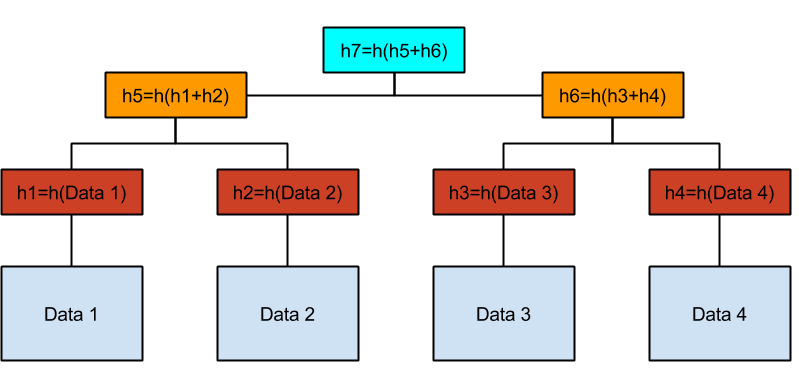
\includegraphics[scale=.4]{merkle_tree}
	\caption{An example of the construction of a Merkle Tree}
	\label{system}
\end{figure}

\section{Implementation}

\subsection{MAST Nodes}

A MAST node is constructed with string content and optional child node pointers. The string content is code that can be executed. A MAST node can have any number of children, each one representing a different branch of program execution, and new branches can be added via the addBr method. Joining all the string content from each node along a path in a MAST therefore yields the code for one possible path of execution for a program.
 
Since branches in a MAST don’t have to be added in any particular order, maintaining the correct Merkle hash for each node during tree construction would be inefficient and require updating previously-set hash values. Instead, that hash function of a MAST node computes the correct Merkle hash using the current state of the tree. It does so by first forming a temporary binary tree of all direct children nodes. As this temp tree is built, hashes are added up to compute a valid Merkle hash at each level of the binary tree. Then, the root hash of the binary tree is summed with the hash of the given node’s content, producing a valid Merkle has for the given node. By including the content hash in the sum, we can ensure integrity of code content later on. Figure 2a shows the temp structure used to calculate the Merkle hash of a given MAST node.

\subsection{Proof Lists}

In order to verify the integrity of code, the MAST function generateFullProofUpward  generates a proof list to a given Merkle root hash from the current node. It does so by crawling upwards in the tree, maintaining a list of the Merkle hashes and code content it passes along the way. The logic gets more complicated due to the fact that Merkle hashes are calculated using a temporary binary tree (as described earlier). As a result, the proof list generator crawls up this binary tree until it hits the parent MAST node, and then repeats the process until the destination node is reached. The content and hashes included in the proof list for a piece of content is shown in Figure 2b

For the verification process, we assume that another machine (without the entire program code) has the Merkle hash of the MAST root node. With a proof list whose destination node is the MAST root hash, this other machine could verify the code in the proof list by iterating over it, summing up the hash values to make sure that they add up to the next hash value in the proof list. If the final summation yields the root hash, then the sequence of hashes provided is correct. Since content hashes get included in the proof list, we can also verify the integrity of the code content itself.

\begin{figure}[h]
	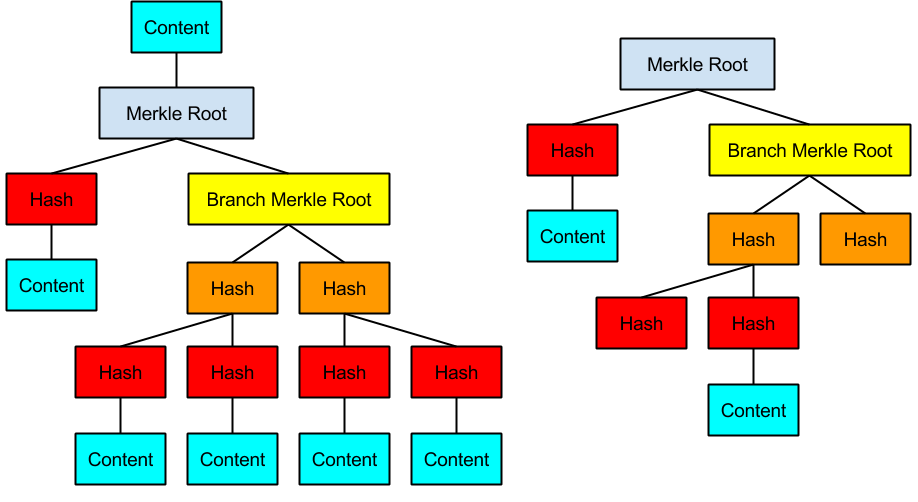
\includegraphics[scale=.35]{mast}
	\caption{Some examples demonstrating functionalities of  the MAST: the recursive data structure(left) and a proof for a particular branch of execution for a MAST(right)}
	\label{system}
\end{figure}

\subsection{Consensus Protocol Simulation}

We implemented a crypto currency network simulator to use MASTs to verify and execute code transferred over the network. To simulate the transaction verification process used in Bitcoin, we created ConsensusNodes to execute and validate the code in a transaction. There are three different types of ConsensusNodes: GoodNodes, EvilNodes, and InconsistentNodes. GoodNodes execute code properly and include transactions in their local ledgers if they are valid. EvilNodes do the opposite, adding invalid transactions to their ledgers and excluding valid ones. InconsistentNodes behave correctly with some probability. With the three node types, we can simulate more realistic network conditions and the presence of adversaries.

Code for a transaction is stored in a MAST, and the transaction saves its root Merkle hash. The compression MASTs offer reduces the amount of data that has to be transferred between nodes during validation. Using an args array, we support passing arguments to transaction code and specifying the subsequent transaction to be run. Transactions also have associated amounts that are used to check whether the code is valid. A valid transaction is one whose amount is at least as large as the sum of amounts of its subsequent transactions.

After individual nodes validate/invalidate a set of transactions, the GlobalConsensus node determines the final outcome of a transaction; a transaction is valid if a majority of the ConsensusNodes validate it. The GlobalConsensus node updates a global ledger representing the correct state of the system, and ConsensusNodes can sync with this ledger to maintain an accurate picture of state.

\section{Applications and Experiments}

\subsection{Contractual Agreements}

Using the previously discussed consensus protocol, we implemented a contract modeling a will that utilized the shared contract creation, verification, and execution functionalities of the MAST to create a multiparty execution environment. The will-based contract we implemented consisted of an agreement between three parties: Alice, Bob, and Carol. The branches of the tree represent approved expenditures both before and after Alice’s death, and present clauses of the contract as a series of branches that are unlocked upon the fulfillments of certain conditions in conjunction with the signatures of relevant signatories. This structure allows for sub-contracts to exist within the subset of the primary signatories and enables full transparency of the content of the contract while restricting execution of certain clauses to when necessary preconditions are satisfied.

The consensus protocol to verify valid construction and execution of the will was implemented using a group of Nodes (comprised of representative ConsensusNodes from the GoodNode, BadNode, and InconsistentNode classes discussed above) which each verified the validity of a transaction.

\subsection{Code Compression}

The primary benchmarks used to quantify code compression were a series of python scripts, which can be found in our repo at the location MAST/bin. The file longcode.py (Figure 3, next page) generates a Merkle tree with tens of thousands of branches, yielding a total code length of 2M characters, The post-compression result after applying our algorithms was under 23,500 characters, indicating a compression rate of over 98\%. We cannot compare the code compression we saw directly to compressing with another algorithm such as LZW because such algorithms employ frequency based compression and longcode uses repeated segments again and again This is OK to do because we are doing a structural compression. Instead, we compared it to using zip to compress the Linux kernel. This took it from roughly 6115332 characters in length to 1754665 characters, a compression rate of 70\%. It is important to note that compression algorithms could also be used in several places in MASTS as well: per code block, and on the complete proof. Additionally, we use an unoptimized message format to send MASTS which is essentially a list of $[([subproof],data, mroot) ]$ which could be further optimized to rely on less punctuation and whitespace and use more efficient character encodings.

\begin{figure}[t!]
	\lstinputlisting[language=Python, breaklines=true]{../bin/longcode.py}
	\caption{An example demonstrating code compression on a Merkle tree with millions of characters. Conversion to a MAST representation yielded a compression score of over 98.9\%}
\end{figure}

\section{Significance and Future Work}

The primary impact of this projects is in its applications to established environments utilizing contracts. The introduction of MASTs has potential to greatly impact existing problems ranging from bitcoin contracts to code transfer between distributed nodes on a network. Potential improvements to this implementation of the MAST could include greater support for distributed construction and execution or the addition of a framework allowing greater extensibility by users of this data structure.

\pagebreak

\bibliographystyle{abbrv}
\bibliography{paper}

\end{document}
